\subsection{L4: Autonomy in Deployment and Environmental Adaptation}

At L4, AI uses feedback from continued deployment interaction to decide
how the operating agent should persistently adapt.
Whereas L3 centers on what experience to acquire for learning, L4 centers
on how operational experience changes the memory, skills, or execution
components used in subsequent tasks.
Retained changes shape later behavior and the feedback available for
further adaptation.
The objective, access boundaries, protected evaluation, and authority
over consequential releases remain externally governed. 
Figure~\ref{fig:L4} provides an overview of this deployment-adaptation
mechanism, showing how interaction experience is converted into persistent
changes that shape subsequent behavior.

The characteristic loop at this level can be summarized as follows:

\begin{center}
\fcolorbox{black!25}{gray!4}{%
\begin{minipage}{0.92\linewidth}
\centering
\vspace{6pt}

\LoneStep{observe deployment interaction}
\(\;\longrightarrow\;\)
\LoneStep{propose persistent adaptation}
\(\;\longrightarrow\;\)
\LoneStep{revise agent components}

\vspace{7pt}

\(\;\longrightarrow\;\)
\LoneStep{validate and retain}
\(\;\longrightarrow\;\)
\LoneStep{reuse in later tasks}
\(\;\longrightarrow\;\)
\LoneStep{collect new feedback and repeat}

\vspace{6pt}
\end{minipage}%
}
\end{center}

We organize the discussion around trajectory distillation, iterative
revision of the agent system, and selective retention and deployment of
updates. These mechanisms differ in what they change, when the change is
reused, and how continued usefulness is established.
Table~\ref{tab:l4-adaptation-summary} summarizes representative methods
along these three axes.

\begin{figure*}[!t]
    \centering
    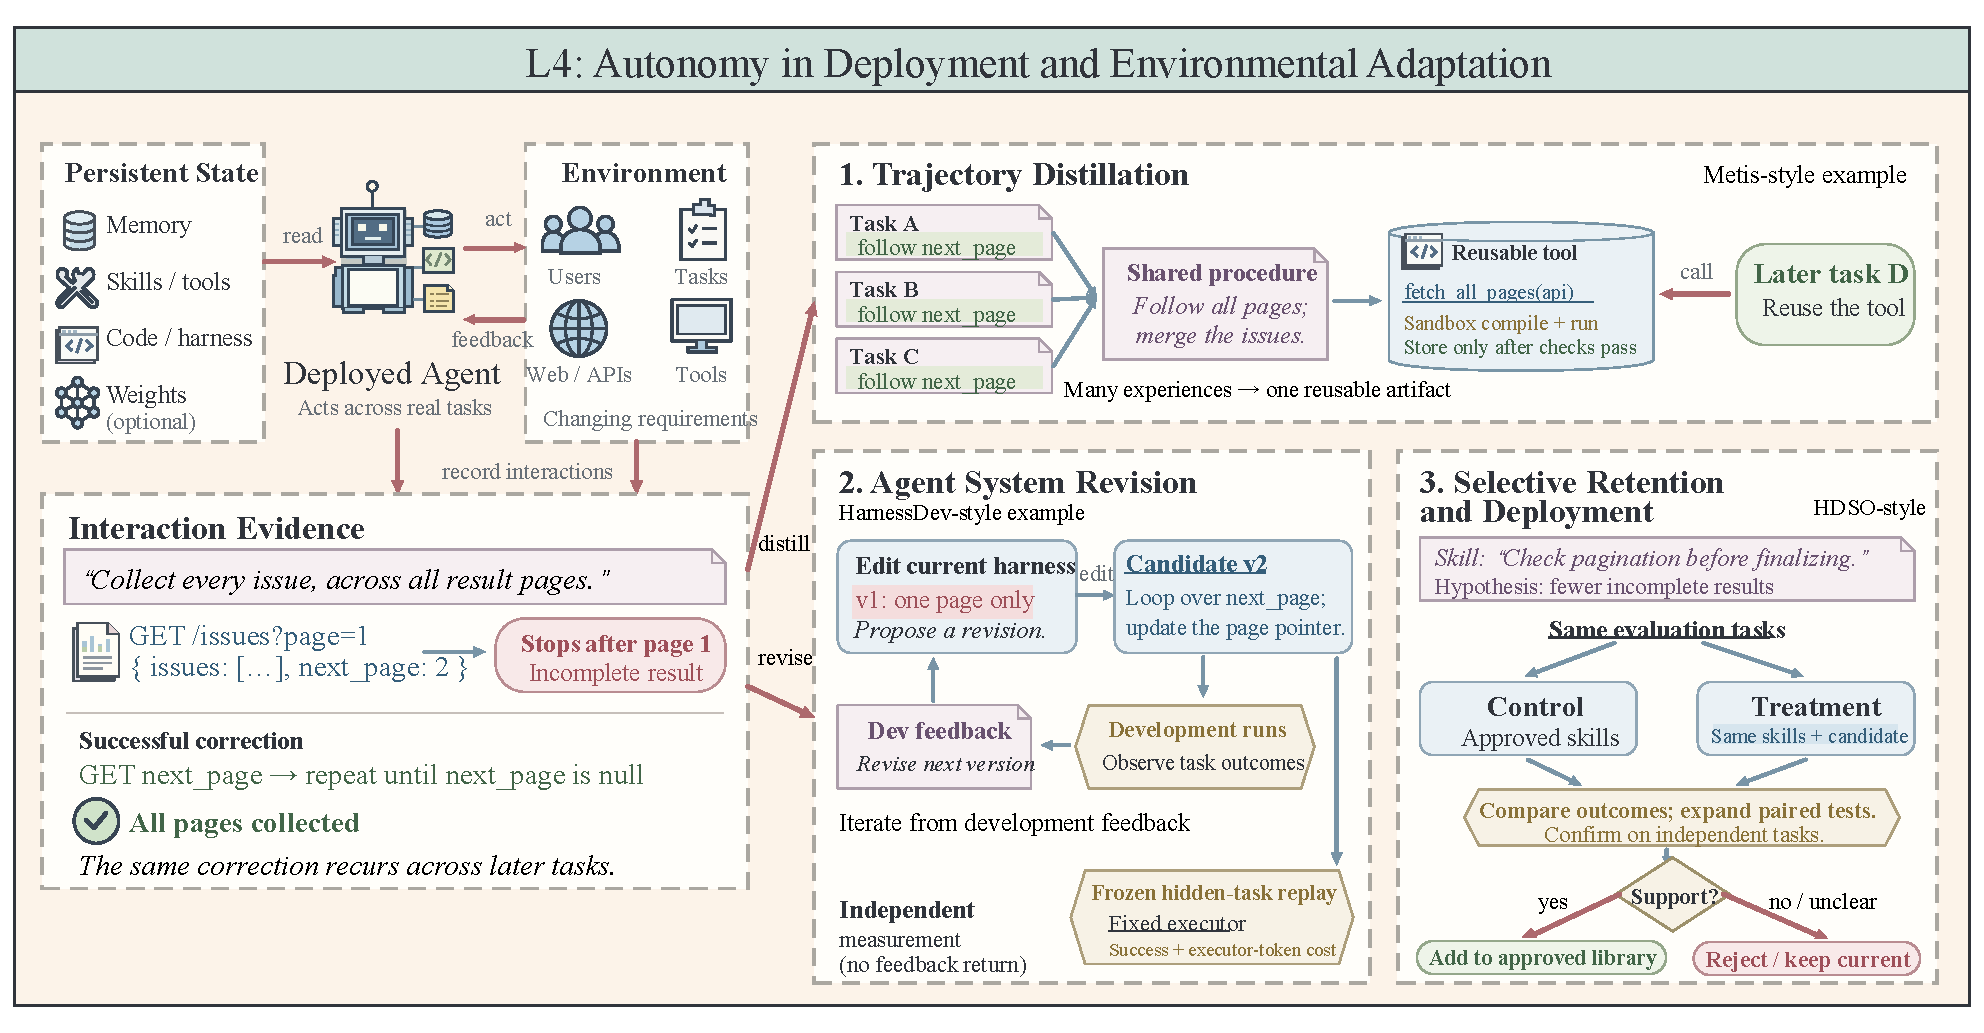
\includegraphics[width=1\linewidth]{figures/L4-v2.pdf}
    \caption{Overview of L4: Autonomy in Deployment and Environmental Adaptation.
Under human-defined objectives and deployment constraints, the AI system
uses interaction evidence from real tasks and changing environments to
determine which consequences of experience should persist and influence
future behavior. Experience can be distilled into reusable artifacts,
used to revise persistent components of the agent system, and selectively
retained based on subsequent evaluation. Accepted updates are reused in
later tasks, closing a persistent adaptation loop between deployment
experience and future behavior.}
    \label{fig:L4}
\end{figure*}



\begin{table*}[t]
\centering
\caption{Representative systems, benchmarks, and analyses for L4 adaptation, grouped by the mechanisms discussed in this section.}
\label{tab:l4-adaptation-summary}
\scriptsize
\setlength{\tabcolsep}{3pt}
\renewcommand{\arraystretch}{1.12}
\begin{tabularx}{\textwidth}{@{}>{\raggedright\arraybackslash}p{0.15\textwidth}>{\raggedright\arraybackslash}p{0.23\textwidth}>{\raggedright\arraybackslash}p{0.14\textwidth}>{\raggedright\arraybackslash}X@{}}
\toprule
\textbf{Method} & \textbf{Update target} & \textbf{Timing} & \textbf{Update validation} \\
\midrule
\multicolumn{4}{@{}l}{\textbf{Trajectory distillation}} \\
Dynamic Cheatsheet~\cite{suzgun2026dynamic}
& Evolving text memory
& After each problem
& Task outcomes guide self-curation; no held-out gate. \\
ACE~\cite{zhang2026agentic}
& Incremental context entries
& After each task
& Helpfulness and harmfulness counters guide edits. \\
ReasoningBank~\cite{ouyang2026reasoningbank}
& Reasoning strategies (text)
& After each task
& A judge labels trajectories before strategy extraction. \\
APEX~\cite{li2026apex}
& Milestone dependency graph
& After each episode
& Episode outcomes are propagated through the graph. \\
PersonaAgent~\cite{zhang2026personaagent}
& Per-user persona prompt
& Across user interactions
& No separate admission test is reported. \\
PAHF~\cite{liang2026learning}
& User preference entries
& When requests are ambiguous
& User clarification confirms and revises preferences. \\
MemToolAgent~\cite{er2026memtoolagent}
& Tool-use critiques and retrieval policy
& After tool calls
& Environment and user feedback assess tool use. \\
Trace2Skill~\cite{ni2026trace2skill}
& Portable skill document
& Offline batch
& Error and success analysts propose and merge patches. \\
PRACTICE~\cite{bai2026practice}
& Embodied skill library
& Offline batches
& Success/failure contrasts and teacher distillation. \\
PANDO~\cite{li2026pando}
& Rules and routines
& Online, in-run
& Confidence-scored admission and demotion. \\
PILOT~\cite{xiao2026pilot}
& Procedures and failure modes
& During long-horizon runs
& Supervisor distillation uses live-run feedback. \\
Metis~\cite{dai2026metis}
& Text plans and code tools
& After completed tasks (asynchronous)
& Repeated reuse plus sandbox compile checks. \\
Evo-Harness~\cite{wei2026evo}
& Harness skill tuples
& After task batches
& Failed or negatively evaluated tasks trigger reflection and edits. \\
SHAPER~\cite{wang2026shaper}
& Planning guidance and context-selection code
& Across task rounds
& Sandbox execution and downstream task outcomes. \\
Evo-Memory~\cite{wei2025evo}
& Accumulated agent memory (benchmark)
& Sequential task streams
& Long-horizon evaluation of memory reuse. \\
\midrule
\multicolumn{4}{@{}l}{\textbf{Iterative revision of the agent system}} \\
DecoEvo~\cite{chen2026decoevo}
& Solver and rubric skills
& Iterative rounds
& Score-independent audits, Pareto-checked. \\
HarnessDev~\cite{wu2026harnessdev}
& Runnable agent harness
& Iterative rounds
& Frozen replay of candidates on hidden tasks. \\
ASPIRE~\cite{wu2026aspire}
& Model weights or harness
& Iterative rounds
& Rollback unless the verified score improves. \\
S3Gym~\cite{shi2026s3gym}
& History, summaries, or model parameters
& Iterative rounds
& Compares update pathways without verifier outcomes. \\
Harness Benefit~\cite{lin2026harness}
& Harness updates and their use (analysis)
& Fixed solve-evolve rounds
& Separates update quality from execution benefit. \\
\midrule
\multicolumn{4}{@{}l}{\textbf{Selective retention and deployment of updates}} \\
HDSO~\cite{shang2026hypothesis}
& Candidate skill packages
& Periodic rounds
& Paired control and treatment executions. \\
Library Drift~\cite{zhang2026library}
& Skill library entries
& Each round
& Low-contribution skills are retired. The library is capped. \\
Rethinking Skill Evolution~\cite{liu2026rethinking}
& Skill edits (analysis)
& Multiple rounds
& Filters edits using task outcomes across rounds. \\
Tax AI~\cite{taxai}
& Product code and evals
& Release cycles
& Targeted and regression tests, then human review. \\
\bottomrule
\end{tabularx}
\end{table*}

% \subsubsection*{\textbf{Scope and definition}}
% An operational definition of RSI must specify the feedback source, the state that can change, and the decisions affected by that change. The interaction may occur in a workspace, an application, a conversation, or a physical environment. A retained update can alter how the agent interprets later observations, selects actions, or constructs subsequent updates. We distinguish three aspects of this definition: persistent adaptation, revision of the improvement procedure, and external acceptance boundaries.

% \paragraph*{Persistent adaptation.}
% Persistent adaptation occurs when feedback changes a part of the system that survives the current episode and influences later tasks. The retained state may contain facts, preferences, procedural knowledge, or execution code. This definition requires a temporal connection between earlier experience and later behavior. A study should therefore identify the point at which an update is written and the later decisions that read it. The strength of the resulting claim depends on the diversity of tasks across which the update remains useful.

% \paragraph*{Revision of the improvement procedure.}
% A stronger form of recursion arises when retained changes affect the procedure used to improve the system. Examples include revising how candidate skills are proposed, how experience is selected, or how internal tests are constructed. Better task performance can follow from any of these changes, but attribution requires a comparison of the update procedure across versions. Relevant outcomes include the number of trials needed to obtain a useful update and the reliability of candidate selection under a fixed budget.

% \paragraph*{External acceptance boundaries.}
% The reviewed systems operate within externally specified objectives and acceptance rules. Application state, executable tests, user requirements, and independent evaluation sets constrain which outcomes count as improvements. Internal tasks or rubrics may change within this boundary. Our method comparison focuses on adaptation outside reinforcement learning and considers external state and evaluation when a framework supports several update mechanisms. Benchmark experiments and production case studies are discussed according to the evidence each provides.

\subsubsection{Trajectory distillation}

Trajectory distillation converts an agent's interaction histories into compact artifacts that persist across sessions and condition later tasks. \wyk{Compared with raw trajectories, distilled artifacts are more concise, less costly to consult, and structured for easier reuse in subsequent tasks.} We group the methods below by the form of the distilled artifact: textual experience memory, structured memory, procedural skill libraries, and executable code.

\noindent\textbf{Textual experience memory.} This category keeps the distilled artifact as natural-language passages that are retrieved into the prompt for later tasks. Dynamic Cheatsheet~\cite{suzgun2026dynamic} enables a frozen model to improve across a series of related problems without access to ground-truth labels. It maintains a single evolving note of strategies, code snippets, and known pitfalls, which the same model consults when answering each incoming problem and curates by adding distilled lessons and removing superseded entries. Agentic Context Engineering~\cite{zhang2026agentic} follows the same recipe while keeping the memory detailed and informative as it grows. It stores short entries with counters that record whether each entry helps or hinders later tasks, and adds small patches rather than rewriting the whole note, which avoids information loss by compression. ReasoningBank~\cite{ouyang2026reasoningbank} adapts the idea to multi-step agents and learns from failures as much as from successes by distilling each judged trajectory into a short, titled strategy that is retrieved before later tasks.

\noindent\textbf{Structured memory.} Instead of free text, structured memory stores experience in explicit records or graphs, making the conditions for reuse inspectable. APEX~\cite{li2026apex} encourages an agent to explore new strategies as its memory grows rather than letting it settle into familiar routines by building a strategy map as a graph of task milestones linked by prerequisite relations. After each episode, the outcome is propagated back along the milestones that led to it, so the map records which paths have worked. A separate step adds promising branches that the agent has not tried, and the agent consults the map at planning time to choose between a known good path and an untried one. Other structures mirror the environment. For instance, PersonaAgent~\cite{zhang2026personaagent} and PAHF~\cite{liang2026learning} instead organize memory around individual users. PersonaAgent translates episodic and semantic user memory into a per-user persona prompt, while PAHF revises preference entries by asking users to clarify an ambiguous request when no relevant preference is found, then integrates their feedback into memory and revises outdated entries. MemToolAgent~\cite{er2026memtoolagent} gives memory a more procedural role by storing critiques of failed tool calls and adjusting how many entries it retrieves per call.

\noindent\textbf{Procedural skill libraries.} Instead of only describing experience, this category extracts reusable skills or standard operating procedures that a later agent follows directly. Trace2Skill~\cite{ni2026trace2skill} turns lessons from individual trajectories into skills that other models and tasks can reuse. It first rolls out a frozen agent on domain tasks. Two analyst roles, one focused on errors and the other on successes, then read the trajectories and propose skill edits, which are merged in stages into a portable skill directory. Because the consolidated document is read directly rather than retrieved for each episode, later agents load it once as part of their instructions. PRACTICE~\cite{bai2026practice} applies the same offline distillation to embodied agents while keeping the skill library consistent as it changes rather than growing unbounded, where a trainable skill learner proposes batch edits that add, refine, merge, or remove entries. The learner first learns basic skill generation and library maintenance from oracle trajectories, then learns failure awareness by contrasting successful and failed trajectories from different executors on the same tasks, and is finally distilled toward a stronger teacher on its own edit distribution. Two other methods acquire skills during execution. PANDO~\cite{li2026pando} improves a web agent during deployment by distilling rules that prevent repeated failures and parameterized routines that replace multi-step browser subgoals from each rollout during deployment, while PILOT~\cite{xiao2026pilot} uses a supervisor to distill procedures and failure modes from a live, long-horizon run, so later sessions start with the accumulated skills.

\noindent\textbf{Executable artifacts.} Moving from text to code, this category compiles experience into artifacts that are invoked directly, combining the flexibility of text memory with the efficiency of executable tools. Metis~\cite{dai2026metis} achieves this through a dual memory, a text store of plans, environment facts, and pitfalls alongside a code library of callable tools. A reflector maintains the text entries, and a frequently reused text plan is rewritten as a callable tool and accepted only after it compiles and runs correctly in a sandbox. Retrieval then covers both text entries and tool descriptions. Evo-Harness~\cite{wei2026evo} broadens the target from single tools to the whole harness, compiling lessons from failed or negatively evaluated tasks into cross-task patterns and task-specific procedures. SHAPER~\cite{wang2026shaper} applies the same idea to embodied agents by evolving textual planning guidance together with a sandboxed Python function that selects the context shown to the planner.

\noindent\textbf{Evaluation protocols.} Evaluation protocols for this family differ in time horizon and in what they count as benefit. Evo-Memory~\cite{wei2025evo} restructures datasets into sequential task streams so that memory accumulation and reuse can be measured over long horizons. PANDO~\cite{li2026pando} instead audits behavior within a run, reporting action repetition, step overhead, and prompt-cache utilization, and Metis~\cite{dai2026metis} relates task quality to execution and construction cost.

\subsubsection{Iterative revision of the agent system}

Rather than what an agent remembers, this section revises the agent system itself: the skills that produce solutions, the rubrics that judge them, the harness that runs them, or the weights underneath. The defining question is which components may change and which acceptance criteria stay fixed while they do. We group the work into co-evolving coupled components, benchmarks that measure self-directed system revision, and evolutionary search under fixed verifiers, followed by analyses of whether revision translates into benefit.

\noindent\textbf{Co-evolving components.} Co-evolution revises two coupled components at once, which raises a circularity problem: if the judge improves alongside the solver, higher scores may reflect an easier judge rather than better solutions. DecoEvo~\cite{chen2026decoevo} addresses this problem by evolving a solver skill and a rubric-generator skill in text space while decoupling their objectives and withholding gold rubrics during optimization. The solver skill is updated from criterion-level rubric feedback. The rubric generator, in contrast, is gated by two score-independent audits: a structural audit checks that the generated rubric covers the task's requirements, and a contrastive audit checks that it discriminates between near-tie responses, with Pareto verification across the two. Because the generator never sees the solver's aggregate score, it cannot improve its standing by making the rubric easier.

\noindent\textbf{Benchmarks of self-directed revision.} Rather than proposing new methods, this line of work measures whether current models can revise their own systems at all. HarnessDev~\cite{wu2026harnessdev} asks whether models can create and improve their own harness, the model-external scaffolding of prompts, tool loops, and execution logic. The creator agent builds a complete harness from a minimal seed and a few development cases and iteratively revises it from downstream feedback. The candidate revisions are frozen and scored on hidden tasks for both success rate and executor-token cost, with the creator and the executor kept separate so that harnesses can be compared under one fixed executor. ASPIRE~\cite{wu2026aspire} asks whether a model can improve itself given only a vague goal. It delegates the choice of data, update method, and validation signal to the agent across both weights and the harness, and a score-gated controller rolls back any change whose verified score does not improve. S3Gym~\cite{shi2026s3gym} restricts the question to the experience channel, withholding verifier outcomes so the agent must judge its own trajectories, and compares raw history, compressed summaries, and parameter training as improvement pathways.

% \noindent\textbf{Search under fixed verifiers.} A complementary direction keeps the evaluator fixed and proposes improvements primarily through search. AlphaEvolve~\cite{alphaevolve} applies this design to algorithm discovery. A sampler assembles each prompt from programs stored in a database of earlier candidates. An ensemble of Gemini models then proposes edits, pairing a fast model for breadth with a stronger one for depth. Automated evaluators run and score every candidate program, and the database's evolutionary algorithm decides which programs seed the next round of prompts. Acceptance is therefore decided entirely by objective scores, and the evaluator configuration remains fixed during each search. This makes improvement easier to attribute than in co-evolving setups, though the claim extends only as far as the fixed tests measure.

\noindent\textbf{Analyses of revision benefit.} Whether revision actually translates into benefit is a question in its own right, and one analysis finds that the two are often conflated. The study behind Harness Updating Is Not Harness Benefit~\cite{lin2026harness} separates two capabilities: producing useful persistent updates, and exploiting them at solve time. Each is measured under a fixed solve-evolve protocol with identical prompts and budgets across several model backbones and three agent benchmarks. Updating ability is largely independent of base model capability, with a small model's updates yielding gains comparable to a frontier model's. The ability to benefit from an updated harness, by contrast, varies non-monotonically, and failures concentrate in two modes: relevant artifacts are not activated, or they are activated but not faithfully followed. A practical consequence is that capability investment belongs in the task-solving agent rather than in the evolver.

\subsubsection{Selective retention and deployment of updates}

Trajectory distillation and system revision both end with a proposed change, while this section focuses on which proposed changes become persistent and which stay available to later tasks. The work below applies this control at three points: before admission, during continued use, and at release into an operational system.

\noindent\textbf{Candidate validation.} A proposed update must produce evidence before it can enter the persistent state. HDSO~\cite{shang2026hypothesis} is designed to prevent skills distilled from noisy trajectories from encoding spurious shortcuts or rules that the executor cannot follow. A curator model observes compact executor traces and proposes a hypothesis with an explicit validation plan, where each candidate is tested by executing the same tasks twice, once with the current approved repository as the control and once with the candidate skill added as the treatment, and the candidate enters the approved repository only when the differences between the two runs support the hypothesis. The comparison runs in stages of increasing size and ends with confirmation on independent tasks. Metis~\cite{dai2026metis}, introduced earlier in the trajectory-distillation section, applies a similar gate after the text plan is already retained in memory, where a text plan becomes executable code only after it recurs across tasks and passes dependency and compilation checks.

\noindent\textbf{Library maintenance.} After admission, attention shifts to the health of the library itself, since skills that were once useful can degrade as tasks and models change. The Library Drift study~\cite{zhang2026library} shows that unbounded accumulation gradually degrades retrieval quality and stalls progress, often before the effect becomes visible in task scores. It proposes lifecycle management with three parts. An append-only evidence log tracks each skill's contribution to task outcomes, and a skill is retired when its measured contribution fades. The number of active skills is capped, so a new skill competes with the entries already present. New skills are also written under a meta-skill, a stored guide that steers how future skills are authored. The study shows that governance choices matter: retiring skills too aggressively performs worse than leaving the library unguided. Meanwhile, another analysis~\cite{liu2026rethinking} finds that carefully filtering skill edits, rather than repeatedly rewriting skills from task outcomes, improves task performance.

\noindent\textbf{Governed deployment.} In production, an incorrect update can affect real users, so a strict gate is needed to prevent unexpected issues. The Tax AI deployment~\cite{taxai} applies such a gate inside a production tax-preparation system, where practitioner corrections drive improvement. Corrections are recorded as structured field-level evidence, and repeated failures are grouped into evaluation targets. A coding agent investigates the trace, evaluations, and repository to implement and validate a fix against targeted and regression evaluations. The loop may change only a bounded part of the product, such as the extraction schema, source selection, tax-engine mapper, and graders. Engineers retain decisions about architecture and product design. Each fix arrives as a pull request for engineering review before release, and cases that the agent cannot resolve are routed back to practitioners. Humans therefore make the final acceptance decision, and the delay introduced by this review is part of the loop's operating cost.


\subsubsection{Evaluating L4 Deployment Autonomy}

Greater autonomy over adaptation after deployment does not by itself establish reliable improvement. An L4 system may retain updates without showing that they remain useful as tasks, environments, or executors change. Evaluation should distinguish the degree of deployment autonomy from the quality of the resulting adaptation process.

A characteristic risk at this level is persistent update failure, where an accepted change may affect many later decisions before its weakness becomes visible. Across different forms of retained state, failure may arise because the system infers the wrong lesson from noisy evidence, applies a sound lesson outside its valid scope, fails to invoke a relevant update, or preserves new behavior at the expense of earlier capabilities~\cite{suzgun2026dynamic,zhang2026library,liu2026rethinking,lin2026harness}. Final task scores alone cannot separate these mechanisms. A credible evaluation must connect each retained change to the evidence that produced it, its later use, and its effects on both new and previously solved tasks.

The current evidence leaves further uncertainty about whether deployment adaptation remains effective over time. Most evaluations cover bounded task streams and limited combinations of models, tasks, and environments, while repeated assessment makes longer studies costly~\cite{ni2026trace2skill,xiao2026pilot,wu2026harnessdev}. Feedback may also be incomplete or endogenous to the loop, as outcome labels can be noisy, evaluators can change with the system, and a useful retained artifact may still fail to influence execution~\cite{ouyang2026reasoningbank,chen2026decoevo,lin2026harness}. Evaluation of L4 should consequently examine adaptation across time and distribution shifts, including the point at which a retained change alters later behavior.

L4 autonomy remains bounded by the surrounding deployment process. The agent may decide how interaction evidence changes persistent state, while humans continue to specify the objective, access boundaries, protected evaluation, and release authority. L4 should concern autonomy over operational adaptation within a deployed system.

\begin{center}
\fbox{
\parbox{0.92\linewidth}{
\textbf{Finding: L4 shifts autonomy from selecting experience to deciding which consequences of experience persist in deployment.}
The agent converts interaction histories into retained changes to memory, skills, harnesses, code, or model parameters, and these changes affect later tasks and feedback. Humans retain the objective, protected acceptance criteria, access boundaries, and final authority over consequential releases.
}}
\end{center}
